\documentclass[margin,line]{resume}

\usepackage[latin1]{inputenc}
\usepackage[english,french]{babel}
\usepackage[T1]{fontenc}
\usepackage{fontawesome}

\usepackage[absolute]{textpos} % Подключите пакет
\usepackage{enumitem}

\usepackage{graphicx,wrapfig}
\usepackage{url}
\usepackage[colorlinks=true, pdfstartview=FitV, linkcolor=blue,
citecolor=blue, urlcolor=blue]{hyperref}
\pdfcompresslevel=9

\begin{document}
{\sc \large Grishin Anton --- Backend Developer} \\
\begin{resume}
  \begin{minipage}[t]{0.55\textwidth}
    \section{\mysidestyle Personal\\Information}
    Grishin Anton \\
    Moscow, Russia \\
    \faLinkedin \space
    \href{https://www.linkedin.com/in/anton-grishin-6966a8362/}{\texttt{anton-grishin}}
    \\
    \faGithub  \space
    \href{https://github.com/alchemmist/}{\texttt{alchemmist}} \\
    \faPaperPlane \space \href{https://t.me/alchemmist}{\texttt{@alchemmist}} \\
    \faPhone \space
    \href{tel:+1234567890}{\color{blue}\texttt{+7(915)067-2638}}  \\
    \faEnvelope \space
    \href{mailto:anton.ingrish@gmail.com}{\color{blue}\texttt{anton.ingrish@gmail.com}}
  \end{minipage}
  \begin{minipage}[H]{0.18\textwidth}
    % 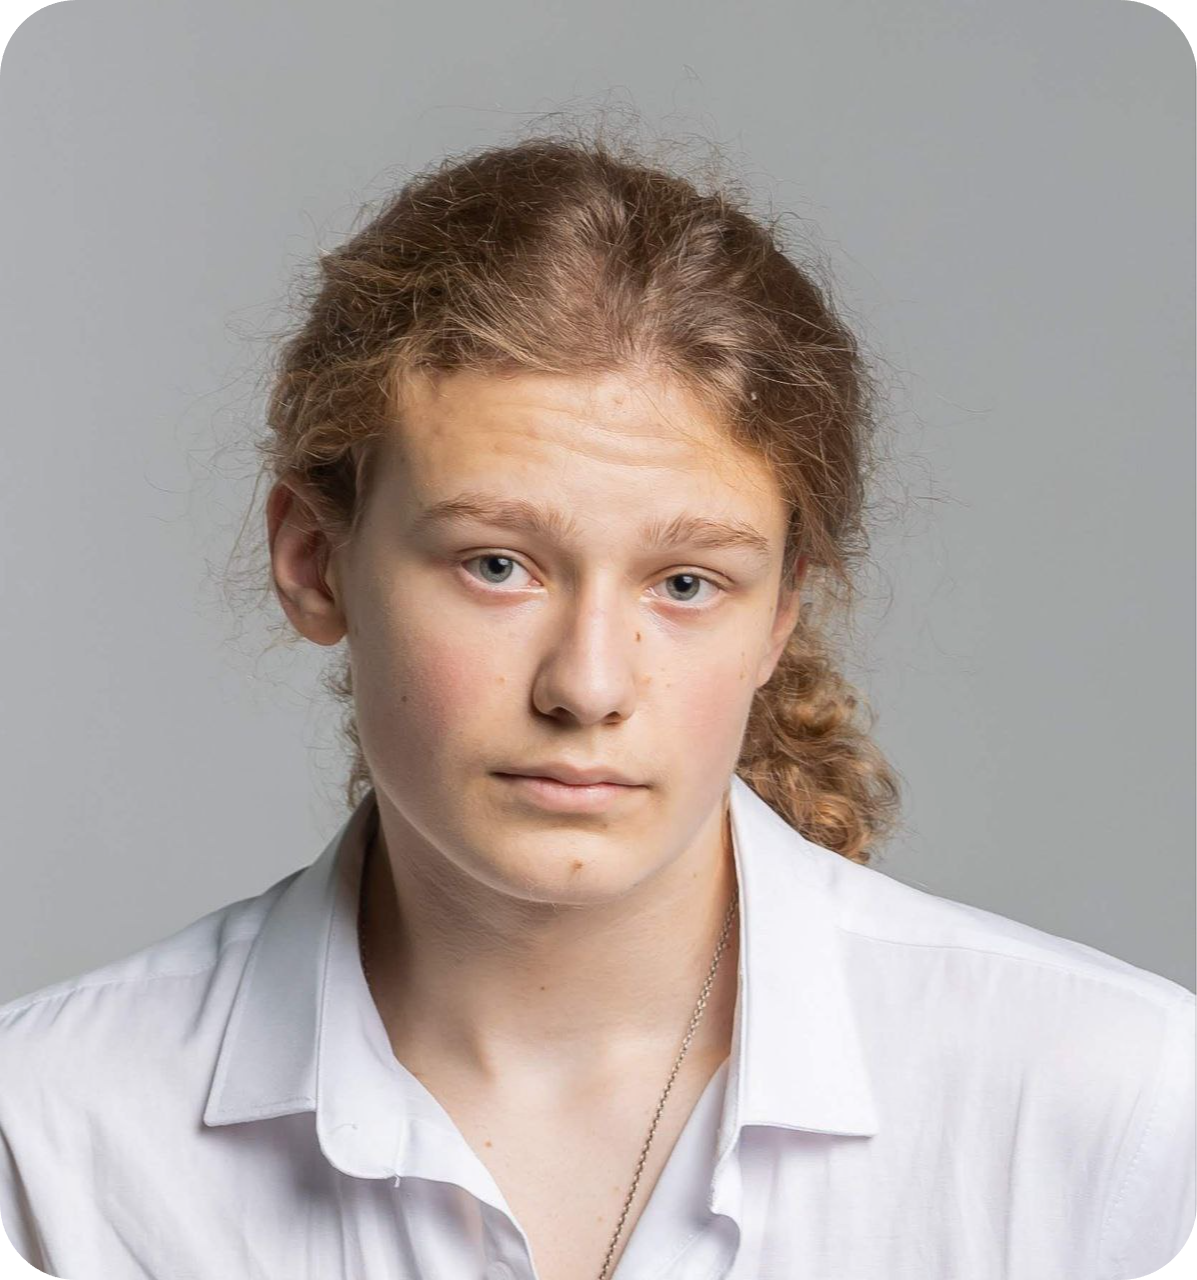
\includegraphics[width=0.45\textwidth]{avatar.png}
    % \hspace{5mm}
    \begin{textblock}{7}(10.54, 1.55)
      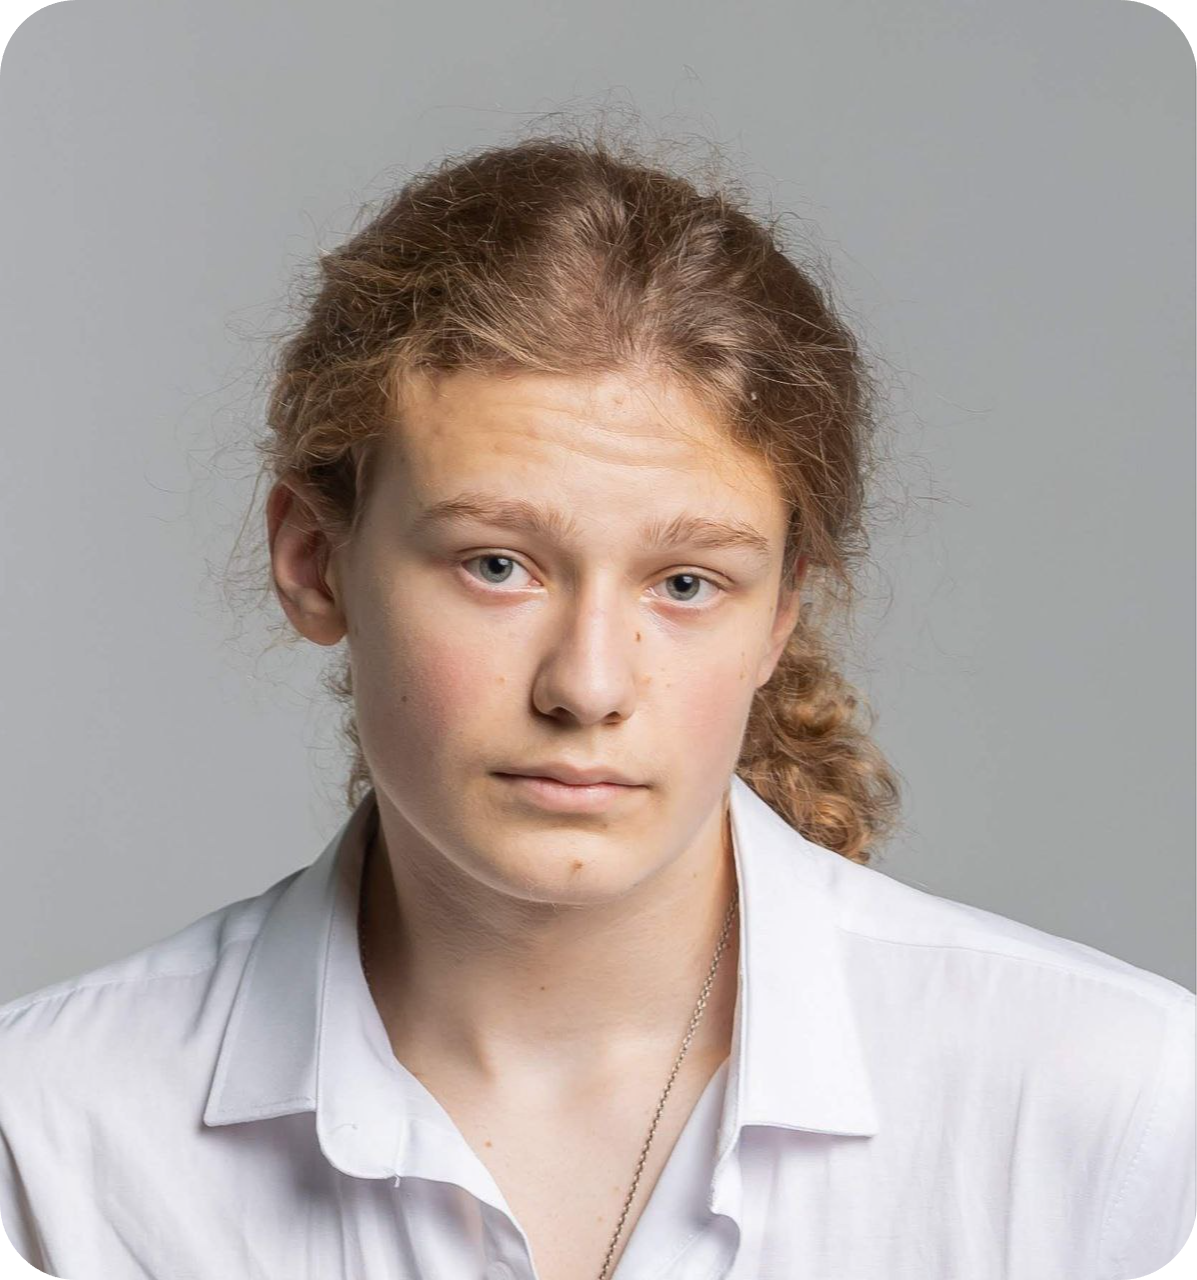
\includegraphics[width=0.27\textwidth]{avatar.png}
    \end{textblock}
  \end{minipage}
  \section{\mysidestyle About me}
  I am a former professional volleyball player, I graduated from the
  Olympic reserve sports school. I also graduated from the
  engineering class at school.

  \section{\mysidestyle Skills}
  \begin{description}[leftmargin=0pt, itemindent=*]
    \item[Python:] FastAPI, Flask, SqlAlchemy, python-telegram-bot,
      faststream, numpy, pandas.
    \item[Go] FastAPI, Flask, SqlAlchemy, python-telegram-bot,
      faststream, numpy, pandas.
    \item[Databases] Postgres, sqlite, Redis, S3(Yandex Object Storage).
    \item[Message brokers:] RebbitMQ, Kafka, Mosquitto.
    \item[Other techonologies:] SQL, Java, JavaScript, Rust, Latex, Go.
    \item[Scientific softwares] Comsys, Maple, Matlab, Mathematica,
      Scilab, Keysight's VEE and ADS, NI LabVIEW.
    \item[Dev tools:] Neovim, Docker, docker-compose, docker-swarm,
      CI/CD(Github actions, GitLab actions)
    \item[Languages:] Russian, English.
  \end{description}

  \section{\mysidestyle Education}
  Central University - Mathematics and Computer Science, 2028

  \section{\mysidestyle Certifications}
  \textbf{Yandex Lyceum.} I was externally admitted directly into the
  second year of the Yandex Academy Lyceum's Industrial Development
  course. I earned a honors certificate and achieved a perfect score
  of 100/100 on the final project.
  \vspace{-6mm}

  \hfill \textsl{September 2022 - April 2023}

  \section{\mysidestyle Achievements}
  \textbf{Qualified for the finals of the Russian Competitive
  Programming Championship}, where our team designed a microservice
  architecture for a web app aggregating sports events across Russia
  (tech stack: RabbitMQ (FastStream), FastAPI, React, Kafka, OAuth)
  and developed an algorithm for processing and validating annual
  government reports on sports events.
  \vspace{-6mm}

  \hfill \textsl{November 2024}

  \textbf{Participated in the Nuclear IT Hackathon}, where my team
  and I worked on a Rosatom case to develop a service for determining
  the emotional tone of online meeting statements. I created
  prototypes and implemented the frontend on React, while my team
  trained the model.
  \vspace{-6mm}

  \hfill \textsl{April 2024}

  \textbf{I won the Science for Life scientific-practical
  conference} with a smart home project for private and public
  educational institutions (tech stack: Redis, Zigbee2MQTT,
  websockets, Go, Python, Flask, React).
  \vspace{-6mm}

  \hfill \textsl{June 2024}

  \section{\mysidestyle Interestings}\vspace{2mm}
  \begin{description}
    \item[Philosophy] Unix, Linux and Windows
    \item[Books:] Unix, Linux and Windows
  \end{description}

  \vfill

  % === HISTORY ===

  \section{\mysidestyle History}\vspace{2mm}

  \begin{description}

    \item[Measurement Engineer (CNRS)]\small{XLIM \hfill \textsl{June
      2016-Present}}\\
    \item[Lecturer]\small{University of Colorado, Boulder \hfill
      \textsl{January 2016-May 2016}}\\
      ECEN 5014-003, ``Microwave Measurements and Calibration Fundamentals''
      \vspace{2mm}

    \item[Research Associate]\small{University of Colorado at Boulder
      \hfill \textsl{June 2013-May 2016}}\\
      Achievements:
      \begin{list2}
      \item{LabVIEW software for a ``Do-it-yourself'' Large-Signal
        Network Analyzer (LSNA)}
      \item{Time domain measurement setup in Scilab (VTD-SWAP)}
      \item{Outphasing PA characterizations}
      \item{Load-pull in time-domain}
      \end{list2}
      \vspace{2mm}

    \item[Measurement Engineer (CNRS)]\small{XLIM \hfill
      \textsl{December 2007-May 2013}}\\
      Achievements:
      \begin{list2}
      \item{Korrigan European Project activities (RTP
            N$^{\circ}$102.052 funded within the EUROPA framework in the
          CEPA2 priority area - ends early 2009) : GaN HEMTs circuits
          level modeling from european foundries (Thales / QinetiQ) for
        HPA, LNA and Switches}
      \item{Time domain measurement setup (LSNA) development on
        Scilab-TCL/TK (GUI, calibration and measurement automation)}
      \item{Development of HEMTs modeling tools (Scilab)}
      \item{Contractual measurements such as load-pull, linearity,
        high impedance probe in both frequency (VNA) and time domain (LSNA)}
      \end{list2}
      \vspace{2mm}

    \item[Research Associate - Visiting Scholar]\small{University of
      Colorado at Boulder \hfill \textsl{February 2012-July 2012}}\\
      GaN HEMTs based rectifiers characterizations and analysis
      \vspace{2mm}

    \item[Research Engineer (CNRS)]\small{XLIM \hfill \textsl{May
      2005-November 2007}}\\
      Achievements:
      \begin{list2}
      \item{Frequency domain load-pull measurement setup (VNA in
          receiver mode with pulse capabilities) developpemnt with
          Scilab (calibration procedures, measurement automation, data
        processing)}
      \item{Large signal caracterization of transistor (mainly
          european GaN in the framework of Korrigan}
        \item{Korrigan WP3.3 workpackage leader in Korrigan.
            Developpement of a internet database (Php / mySQL) to let
          partners share data and informations}
        \item{GaN HEMTs ``spice-like'' nonlinear models}
        \end{list2}
        \vspace{2mm}

      \item[Research Engineer]\small{NMDG Engineering bvba \hfill
        \textsl{November 2004-February 2005}}\\
        Implementation of the High Impedance Probe module
        (calibration and measurements) in the commercial LSNA
        Software (based on Mathematica)

        \vspace{2mm}

      \item[Postdoctoral scientist]\small{CNES (French Space Agency)
        \hfill \textsl{October 2003-September 2004}}\\
        Development of characterization tools interfaces within the
        free open-source scientific package Scilab

        \vspace{2mm}

      \item[Postdoctoral scientist]\small{CNES (French Space Agency)
        \hfill \textsl{October 2002-September 2003}}\\
        Achievements:
        \begin{list2}
        \item{Large Signal Network Analysis (LSNA) characterizations
          in time-domain}
        \item{Development of a new LSNA module in order to
            investigate time domain waveforms at internal nodes of
            MMICs with high impedance probes (HIP) to validate circuits
          designs and to analyze nonlinear parametric stability}
        \item{Large Signal Network Analysis (LSNA) characterizations
          in time-domain}
        \end{list2}
        \vspace{2mm}

      \item[Researcher]\small{IRCOM / University of Limoges \hfill
        \textsl{October 1998-September 2002}}\\
        Achievements:
        \begin{list2}
        \item{Development of the RF time-domain envelope measurement
          setup (hardware and software)}
        \item{Development of the calibration procedure of the
          time-domain envelope measurement setup}
        \item{Power amplifiers characterizations : Load-pull, IM3, NPR}
        \item{Behavioral modeling of nonlinear devices with memory
          effects for system level}
        \item{Development of a dynamic complex gain model with neural networks}
        \end{list2}
        \vspace{2mm}

      \item[Lecturer]\small{University of Limoges \hfill
        \textsl{October 1998-September 2002}}\\
        RF devices, analog/digital communication systems, signal
        processing, propagation waves...
        \vspace{2mm}

      \item[Postgraduate student]\small{IRCOM / University of Limoges
        \hfill \textsl{February 1998-July 1998}}\\
        Circuits level simulations of IM3 and NPR in order to
        optimize the trade-off between linearity and efficiency

    \end{description}

  \end{resume}
  \end{document}
